\begin{figure}[!htbp]
	  \centering
	  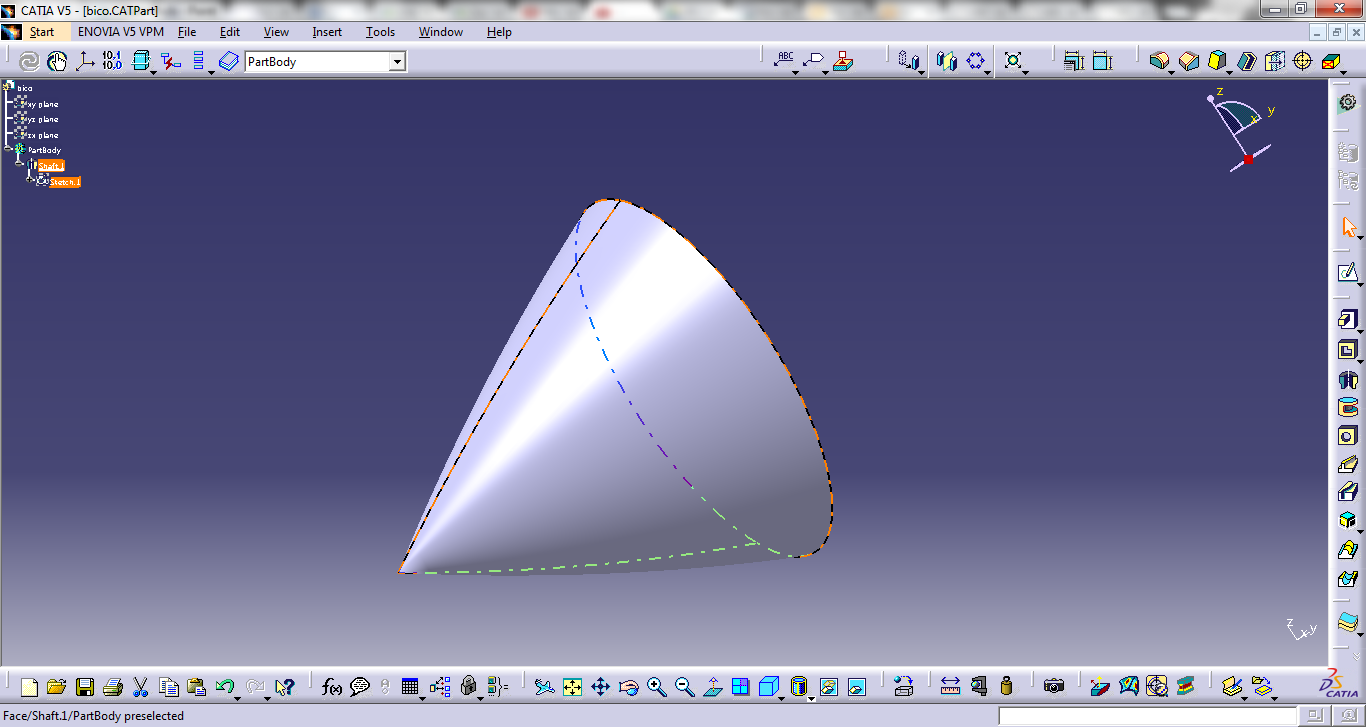
\includegraphics[scale=0.45]{editaveis/figuras/C_Bico}
	  \caption[Bico]{Bico}
	  \label{Bico}
	\end{figure}
	\FloatBarrier
	
\begin{figure}[!htbp]
	  \centering
	  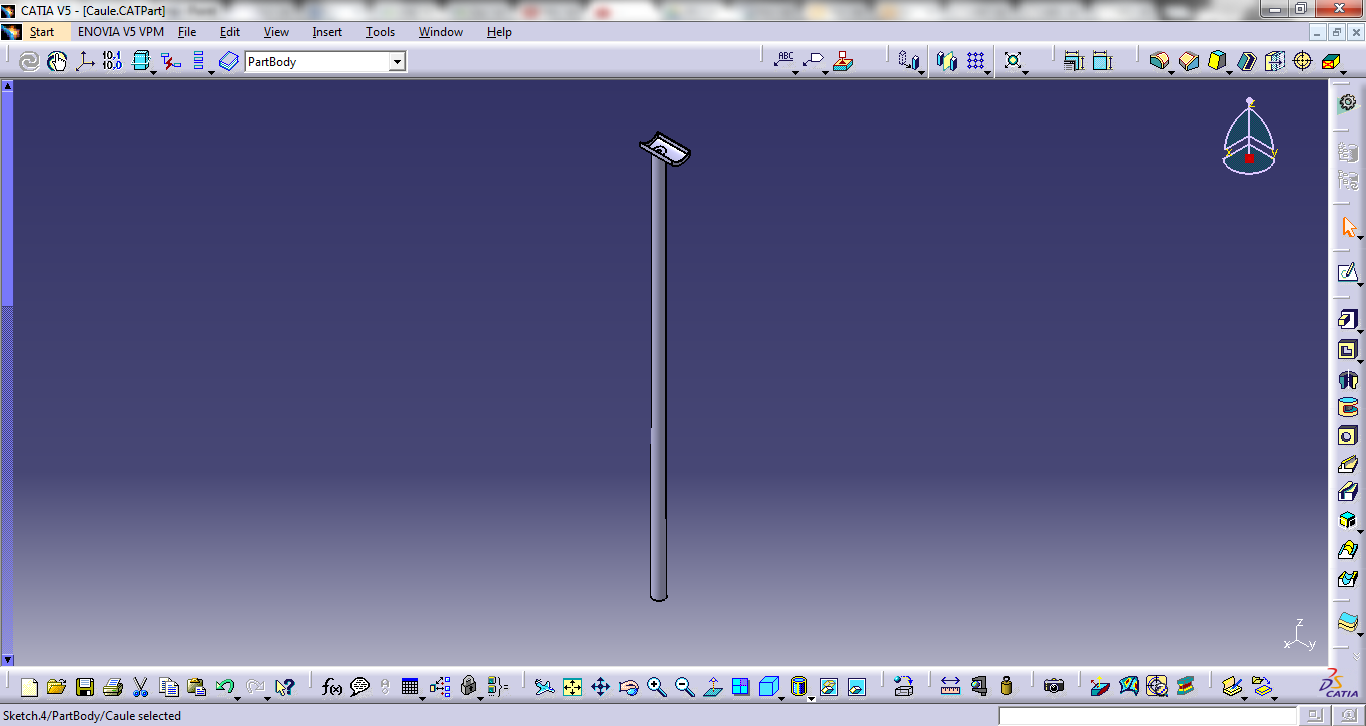
\includegraphics[scale=0.45]{editaveis/figuras/C_Caule_1}
	  \caption[Caule]{Caule}
	  \label{Caule1}
	\end{figure}
	\FloatBarrier
	
\begin{figure}[!htbp]
	  \centering
	  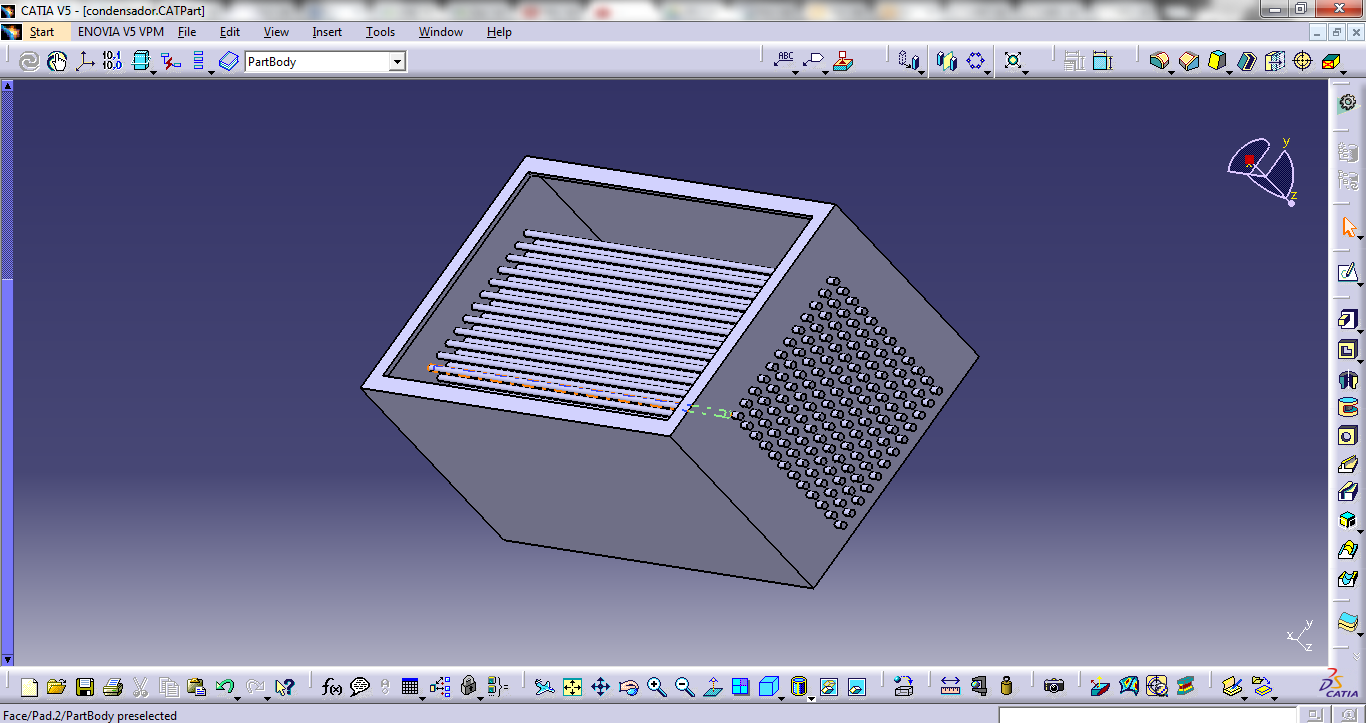
\includegraphics[scale=0.45]{editaveis/figuras/C_condensador}
	  \caption[Condensador]{Condensador}
	  \label{Condensador}
	\end{figure}
	\FloatBarrier
	
	\begin{figure}[!htbp]
	  \centering
	  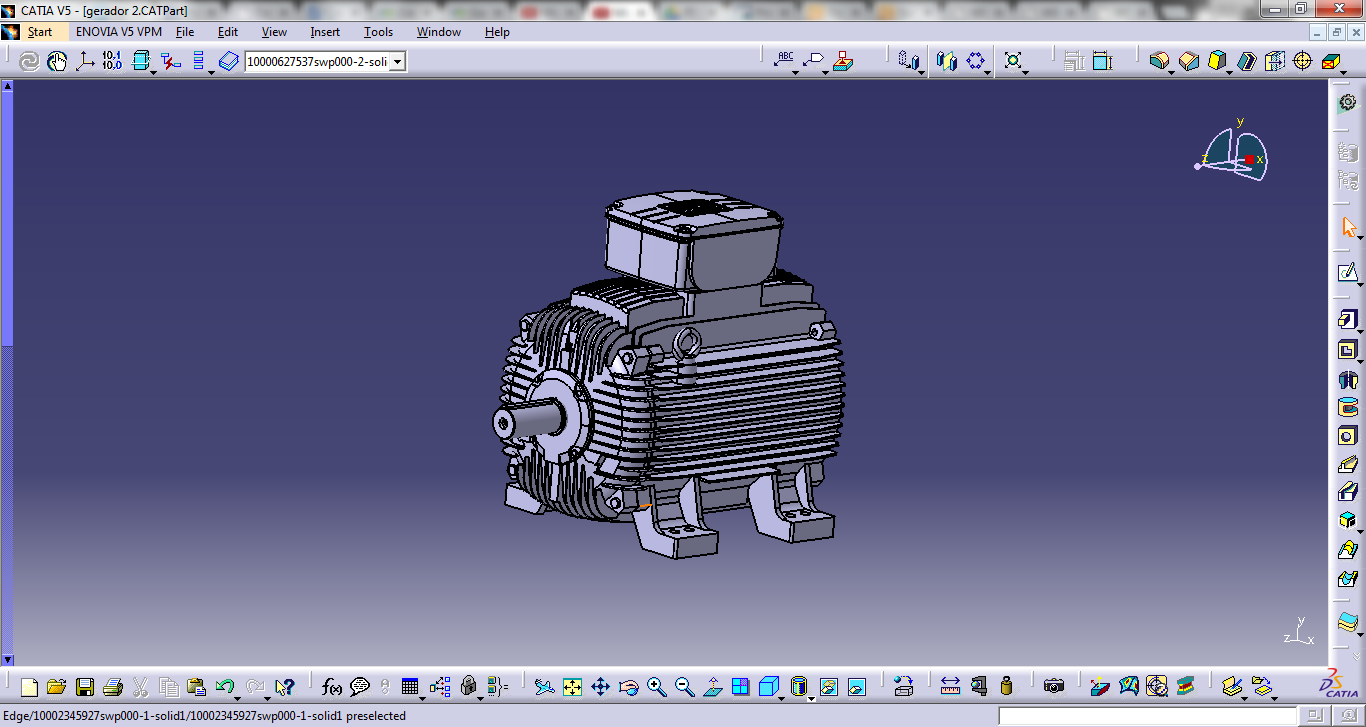
\includegraphics[scale=0.45]{editaveis/figuras/C_Gerador}
	  \caption[Gerador]{Gerador}
	  \label{Gerador}
	\end{figure}
	\FloatBarrier
	
	\begin{figure}[!htbp]
	  \centering
	  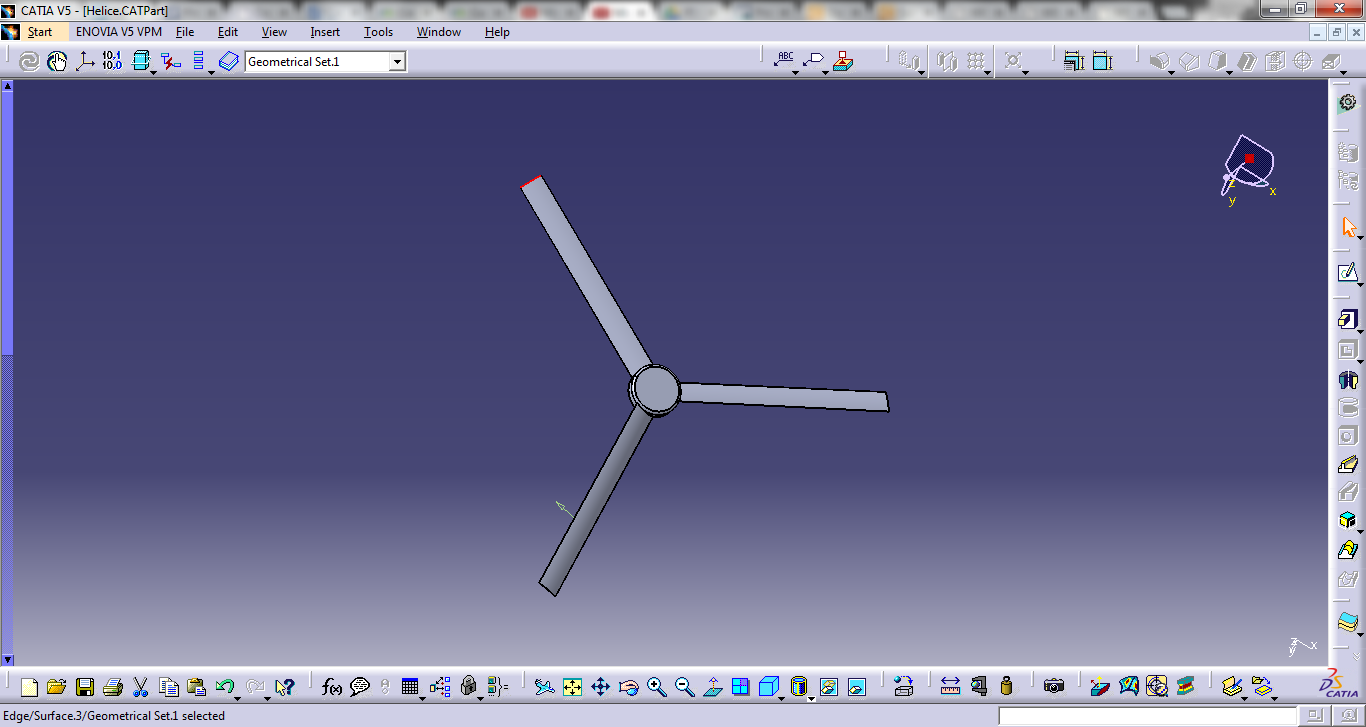
\includegraphics[scale=0.45]{editaveis/figuras/C_helice}
	  \caption[Helice]{Hélice}
	  \label{Helice}
	\end{figure}
	\FloatBarrier
	
\begin{figure}[!htbp]
	  \centering
	  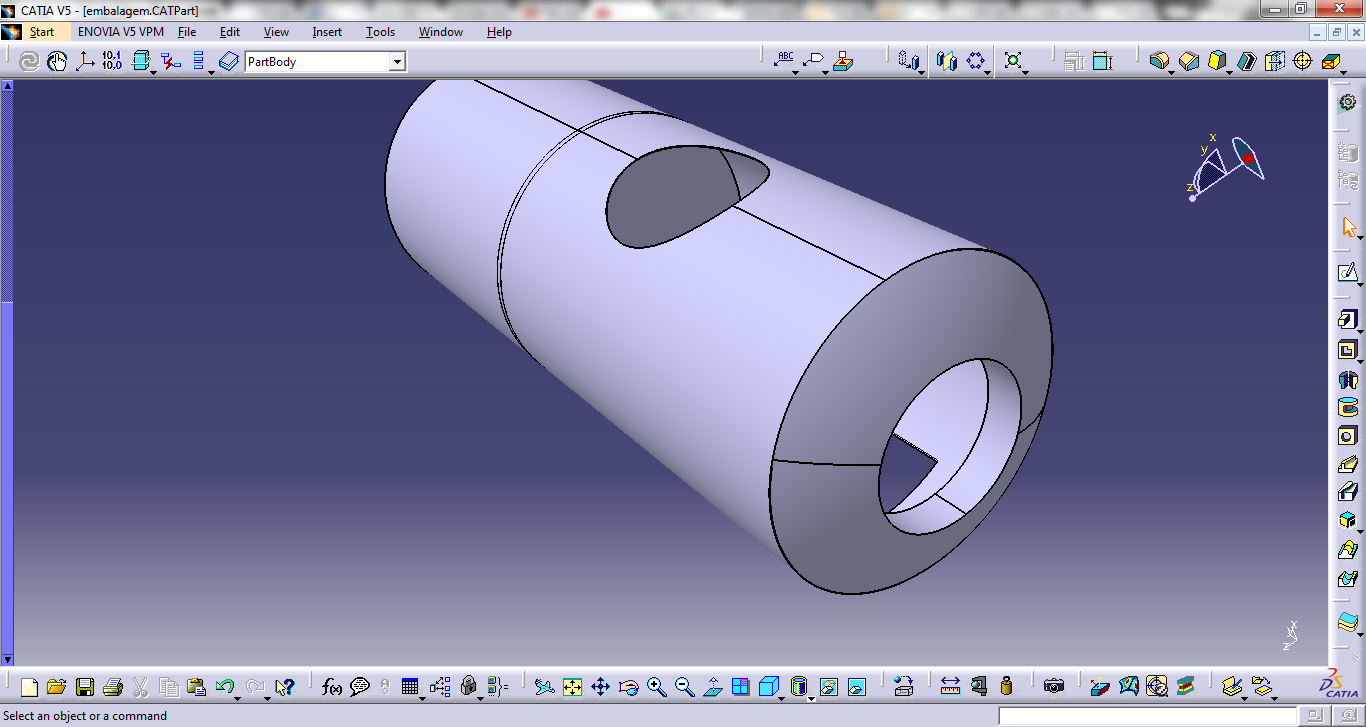
\includegraphics[scale=0.45]{editaveis/figuras/C_Nicele}
	  \caption[Nicele]{Nicele}
	  \label{Nicele}
	\end{figure}
	\FloatBarrier
	
\begin{figure}[!htbp]
	  \centering
	  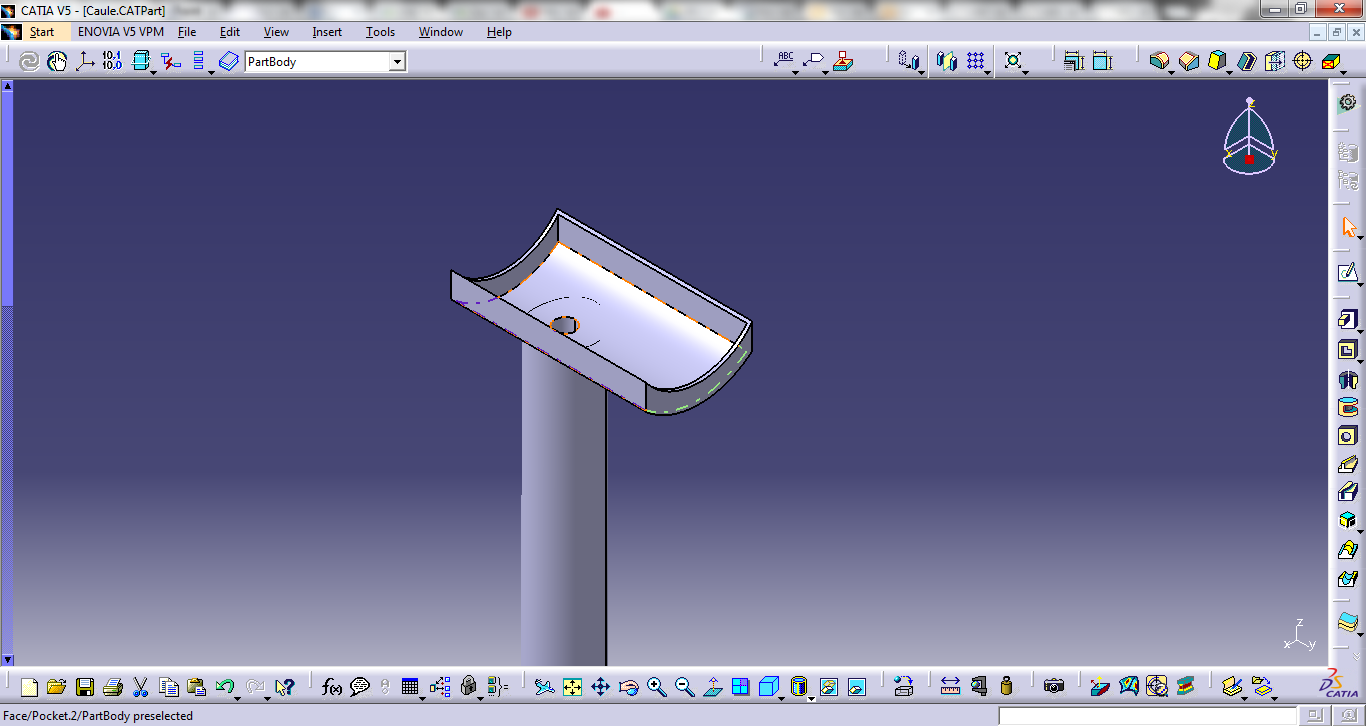
\includegraphics[scale=0.45]{editaveis/figuras/C_Reservatorio}
	  \caption[Reservatorio]{Reservatorio}
	  \label{Reservatorio}
	\end{figure}
	\FloatBarrier
	
\begin{figure}[!htbp]
	  \centering
	  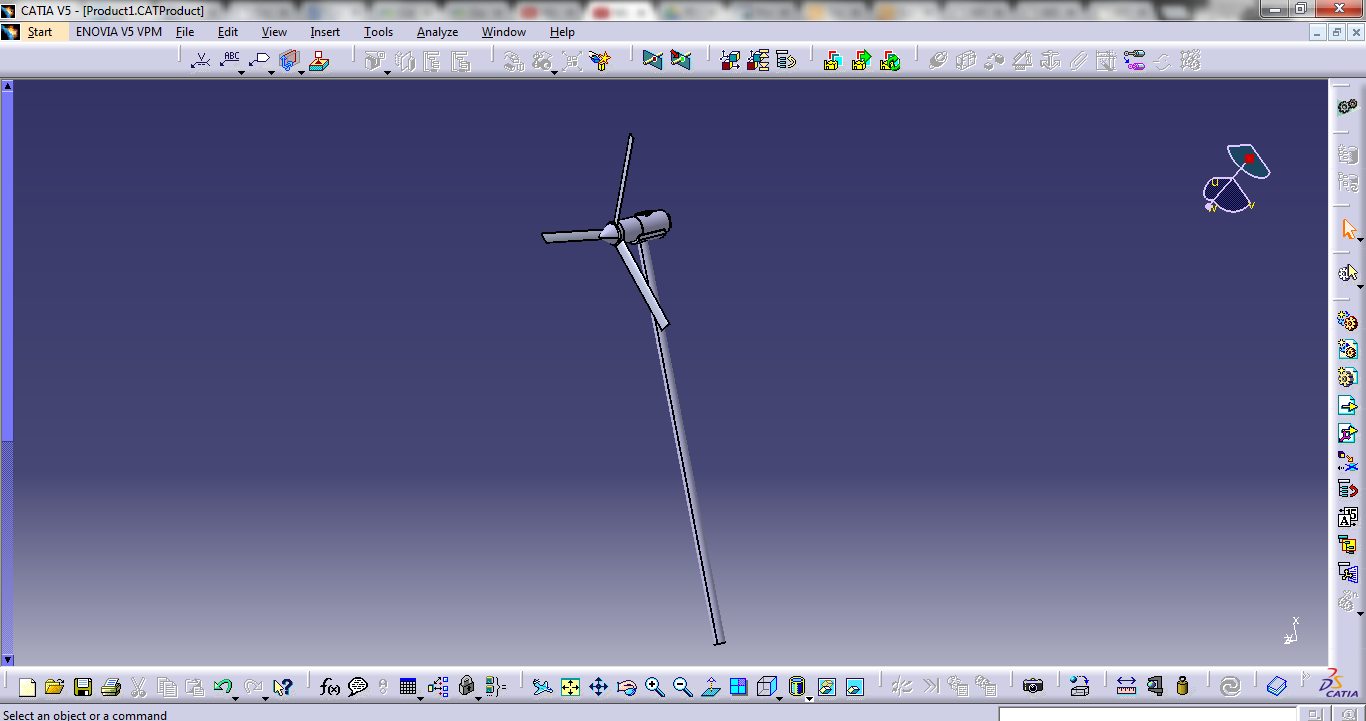
\includegraphics[scale=0.45]{editaveis/figuras/C_torre1}
	  \caption[Torre1]{Torre 1}
	  \label{Torre1}
	\end{figure}
	\FloatBarrier
	
\begin{figure}[!htbp]
	  \centering
	  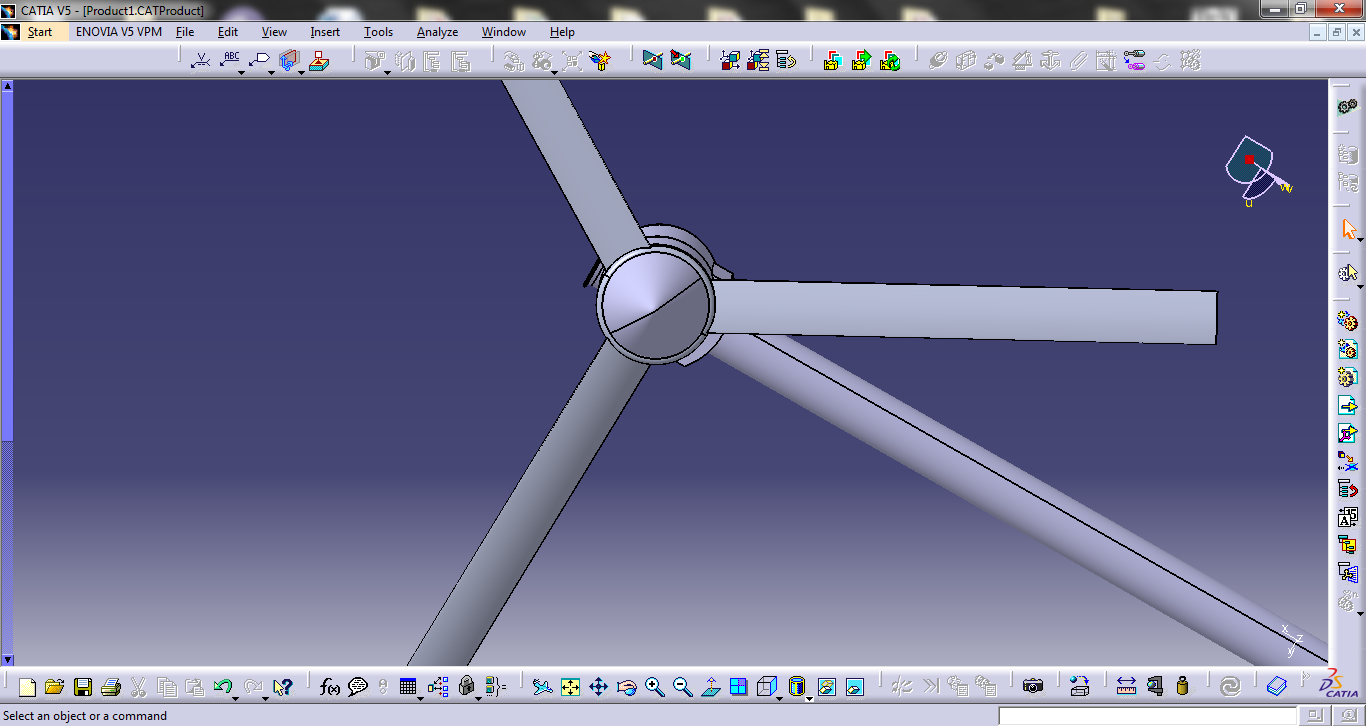
\includegraphics[scale=0.45]{editaveis/figuras/C_torre2}
	  \caption[Torre2]{Torre 2}
	  \label{Torre2}
	\end{figure}
	\FloatBarrier
	
\begin{figure}[!htbp]
	  \centering
	  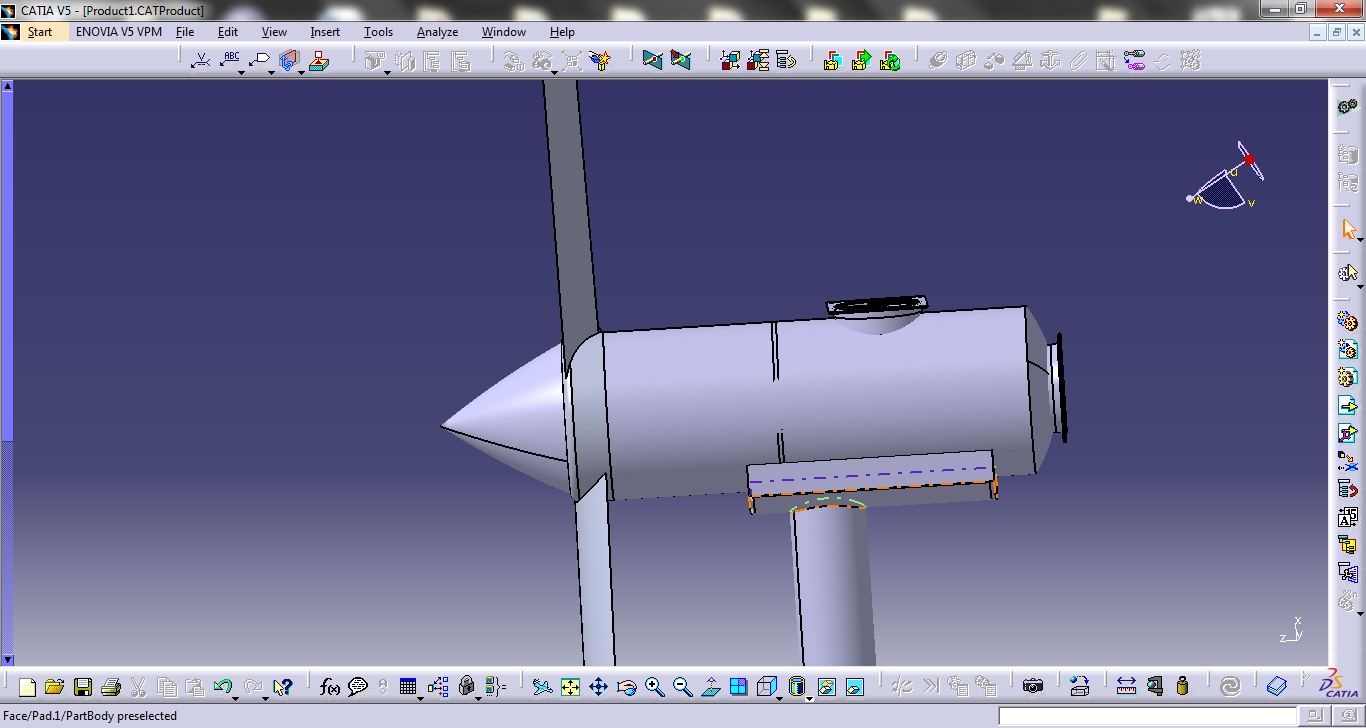
\includegraphics[scale=0.45]{editaveis/figuras/C_torre3}
	  \caption[Torre3]{Torre 3}
	  \label{Torre3}
	\end{figure}
	\FloatBarrier
	
\begin{figure}[!htbp]
	  \centering
	  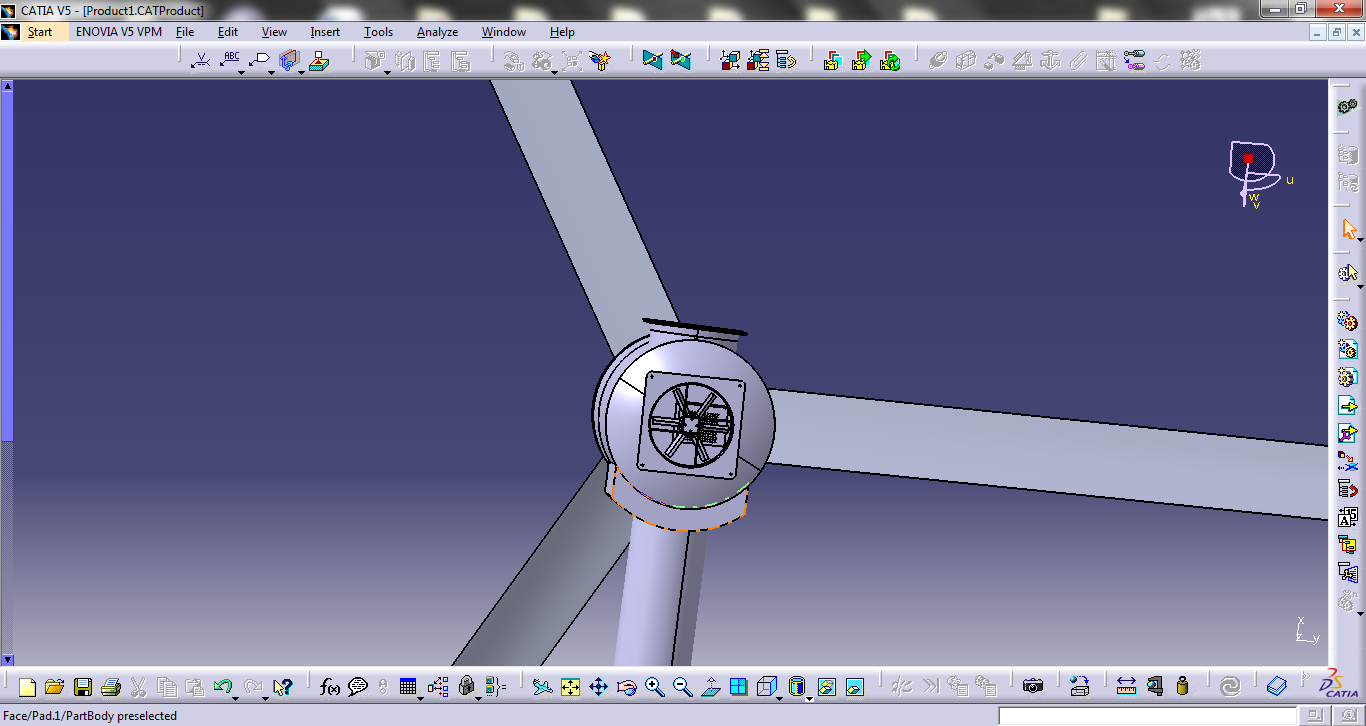
\includegraphics[scale=0.45]{editaveis/figuras/C_torre4}
	  \caption[Torre4]{Torre 4}
	  \label{Torre4}
	\end{figure}
	\FloatBarrier
	
\begin{figure}[!htbp]
	  \centering
	  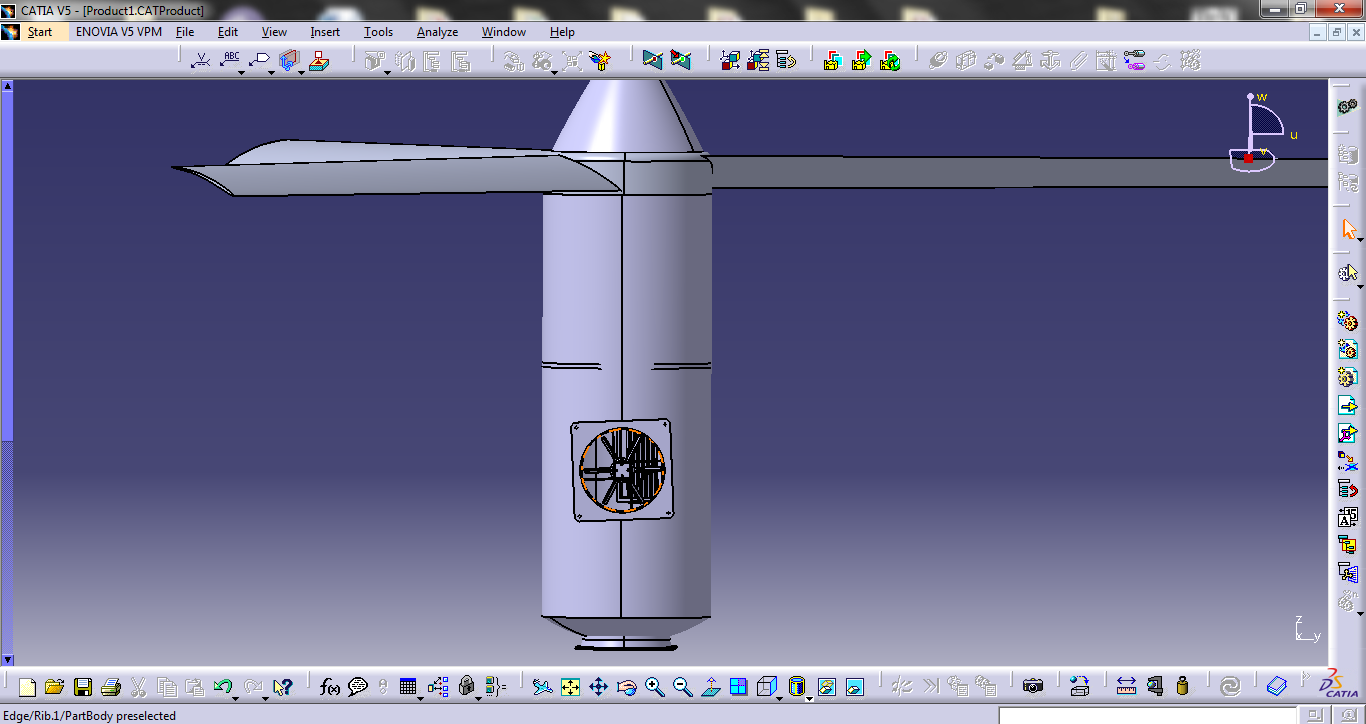
\includegraphics[scale=0.45]{editaveis/figuras/C_torre5}
	  \caption[Torre5]{Torre 5}
	  \label{Torre2}
	\end{figure}
	\FloatBarrier
	
\begin{figure}[!htbp]
	  \centering
	  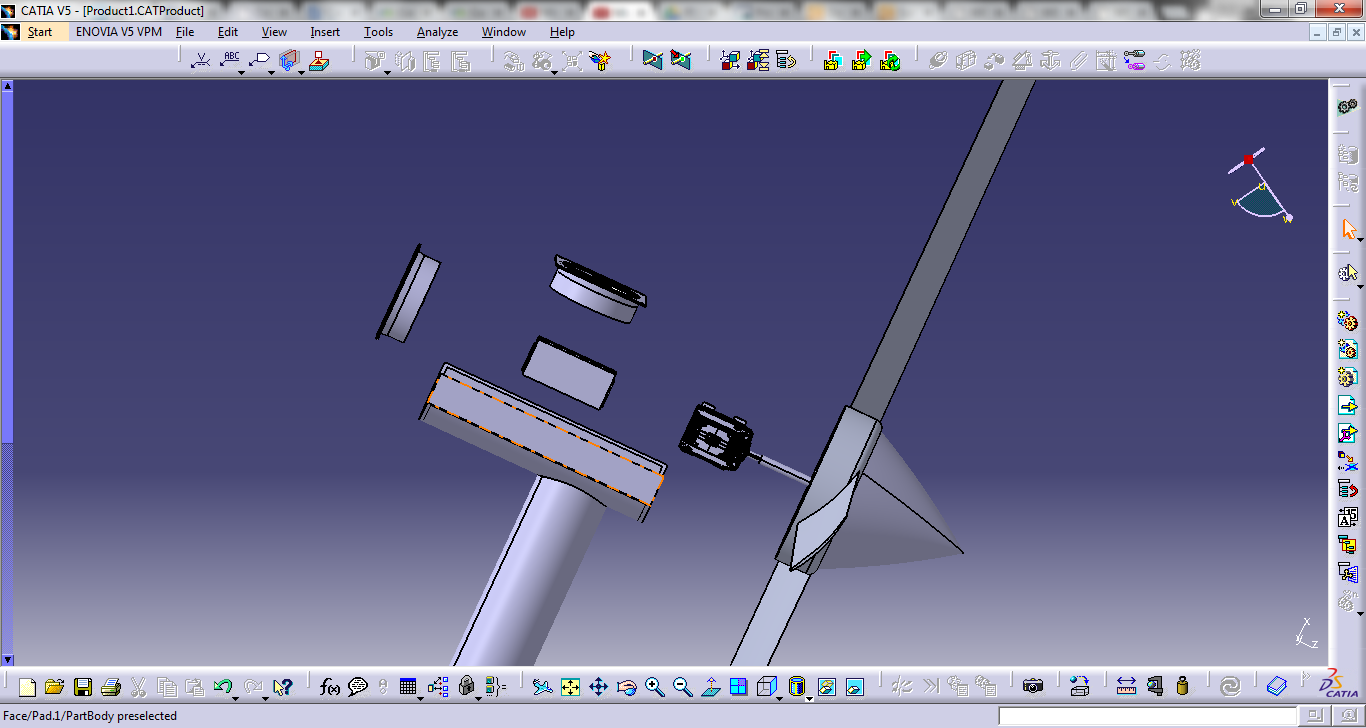
\includegraphics[scale=0.45]{editaveis/figuras/C_torre6}
	  \caption[Torre6]{Torre 6}
	  \label{Torre6}
	\end{figure}
	\FloatBarrier

\begin{figure}[!htbp]
	  \centering
	  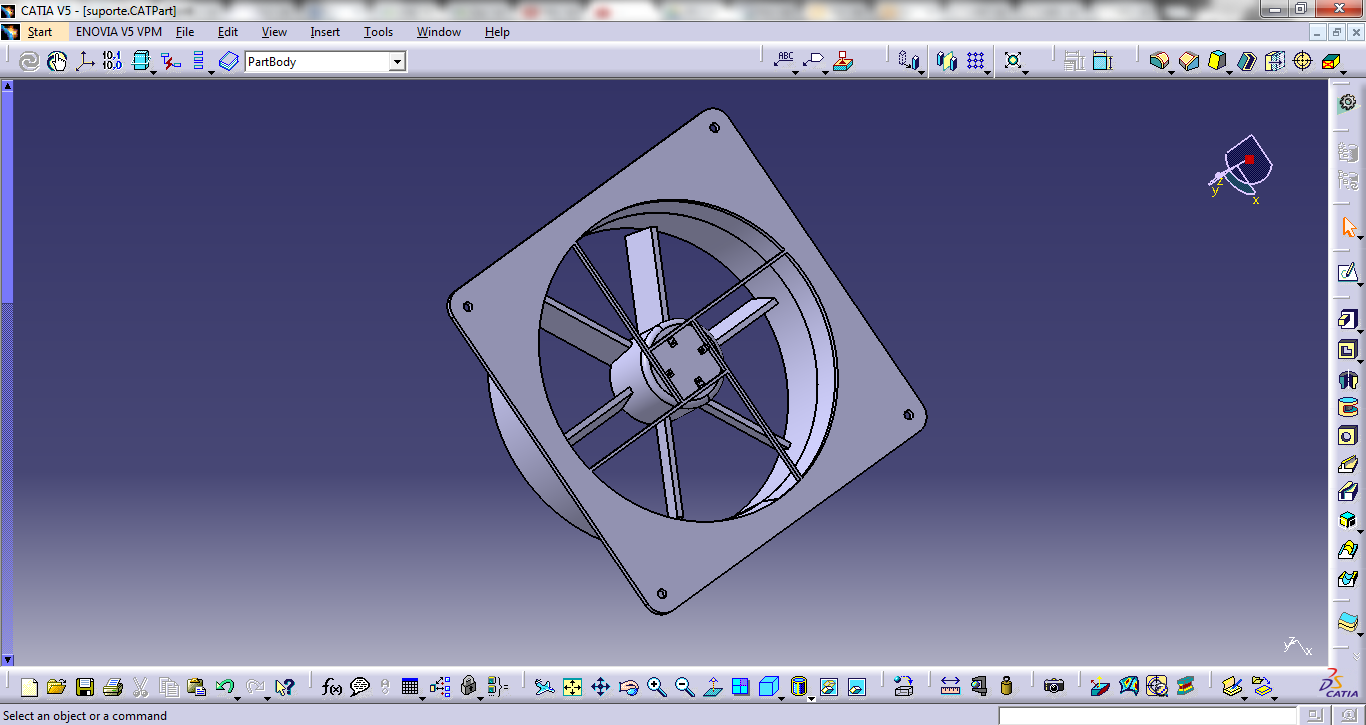
\includegraphics[scale=0.45]{editaveis/figuras/C_Ventoinha}
	  \caption[Ventoinha]{Ventoinha}
	  \label{Torre6}
	\end{figure}
	\FloatBarrier
	